%% Template for the submission to:
%%   The Annals of Applied Statistics [AOAS]
%%
%%%%%%%%%%%%%%%%%%%%%%%%%%%%%%%%%%%%%%%%%%%%%%
%% In this template, the places where you   %%
%% need to fill in your information are     %%
%% indicated by '???'.                      %%
%%                                          %%
%% Please do not use \input{...} to include %%
%% other tex files. Submit your LaTeX       %%
%% manuscript as one .tex document.         %%
%%%%%%%%%%%%%%%%%%%%%%%%%%%%%%%%%%%%%%%%%%%%%%

\documentclass[aoas]{imsart}

%% Packages
\RequirePackage{amsthm,amsmath,amsfonts,amssymb}
\RequirePackage[authoryear]{natbib}
\RequirePackage[colorlinks,citecolor=blue,urlcolor=blue]{hyperref}%% uncomment this for coloring bibliography citations and linked URLs
\RequirePackage{graphicx}%% uncomment this for including figures



%%PACKAGES
\usepackage{caption}
\usepackage{subcaption}
\usepackage{float}
\usepackage{multirow}
\usepackage{lscape}
\usepackage{calc}
\usepackage{array}
\usepackage{bbold}
\usepackage{comment}
\usepackage{xcolor}
\usepackage{nicematrix}
\usepackage{multirow}
\usepackage{diagbox}
\usepackage{tikz}
\usepackage{yhmath}
\usetikzlibrary{quotes,angles}
\usepackage{pgfplots}
\pgfplotsset{compat = newest}
\usepackage{fancyhdr}


% set up for custom R code
\usepackage{listings}
\definecolor{darkgreen}{rgb}{0.0, 0.5, 0.0} % Define a dark green color for the comments

\lstdefinestyle{customR}{
	language=R,
	backgroundcolor=\color{lightgray},
	basicstyle=\ttfamily\footnotesize,
	keywordstyle=\bfseries\color{blue},
	commentstyle=\itshape\color{darkgreen}, % Use the custom dark green color
	stringstyle=\color{red},
	numbers=left,
	numberstyle=\tiny\color{gray},
	stepnumber=1,
	numbersep=10pt,
	showspaces=false,
	showstringspaces=false,
	showtabs=false,
	frame=single,
	rulecolor=\color{black},
	tabsize=2,
	captionpos=b,
	breaklines=true,
	breakatwhitespace=false,
	title=\lstname,
	escapeinside={\%*}{*)},
	morekeywords={*,...} % if you want to add more keywords to highlight
}

\lstset{style=customR}


\startlocaldefs
%%%%%%%%%%%%%%%%%%%%%%%%%%%%%%%%%%%%%%%%%%%%%%
%%                                          %%
%% Uncomment next line to change            %%
%% the type of equation numbering           %%
%%                                          %%
%%%%%%%%%%%%%%%%%%%%%%%%%%%%%%%%%%%%%%%%%%%%%%
%\numberwithin{equation}{section}
%%%%%%%%%%%%%%%%%%%%%%%%%%%%%%%%%%%%%%%%%%%%%%
%%                                          %%
%% For Axiom, Claim, Corollary, Hypothesis, %%
%% Lemma, Theorem, Proposition              %%
%% use \theoremstyle{plain}                 %%
%%                                          %%
%%%%%%%%%%%%%%%%%%%%%%%%%%%%%%%%%%%%%%%%%%%%%%
%\theoremstyle{plain}
%\newtheorem{???}{???}
%\newtheorem*{???}{???}
%\newtheorem{???}{???}[???]
%\newtheorem{???}[???]{???}
%%%%%%%%%%%%%%%%%%%%%%%%%%%%%%%%%%%%%%%%%%%%%%
%%                                          %%
%% For Assumption, Definition, Example,     %%
%% Notation, Property, Remark, Fact         %%
%% use \theoremstyle{remark}                %%
%%                                          %%
%%%%%%%%%%%%%%%%%%%%%%%%%%%%%%%%%%%%%%%%%%%%%%
%\theoremstyle{remark}
%\newtheorem{???}{???}
%\newtheorem*{???}{???}
%\newtheorem{???}{???}[???]
%\newtheorem{???}[???]{???}
%%%%%%%%%%%%%%%%%%%%%%%%%%%%%%%%%%%%%%%%%%%%%%
%% Please put your definitions here:        %%

\newtheorem{theorem}{Theorem}[section]
\newtheorem{corollary}{Corollary}[section]
\newtheorem{lemma}{Lemma}[section]
\newtheorem{proposition}{Proposition}[section]

\theoremstyle{definition}
\newtheorem{definition}{Definition}[section]

\theoremstyle{remark}
\newtheorem*{remark}{Remark}
\theoremstyle{remark}
\newtheorem*{example}{Example}

%% SHORTCUTS
\DeclareMathOperator{\diag}{diag}
\DeclareMathOperator{\Span}{span}
\DeclareMathOperator{\erf}{erf}
\newcommand {\R}{\mathbb{R}}
\newcommand {\E}{\mathbb{E}}
\newcommand {\prob}{\mathbb{P}}
\newcommand {\N}{\mathbb{N}}
\newcommand {\Z}{\mathbb{Z}}
\newcommand {\1}{\mathbb{1}}


%%%%%%%%%%%%%%%%%%%%%%%%%%%%%%%%%%%%%%%%%%%%%%

\endlocaldefs

\begin{document}

\begin{frontmatter}
%%%%%%%%%%%%%%%%%%%%%%%%%%%%%%%%%%%%%%%%%%%%%%
%%                                          %%
%% Enter the title of your article here     %%
%%                                          %%
%%%%%%%%%%%%%%%%%%%%%%%%%%%%%%%%%%%%%%%%%%%%%%
\title{Supplementary file to "Varying coefficients correlated velocity models in complex landscapes with boundaries applied to narwhal responses to noise exposure"}
%\title{A sample article title with some additional note\thanksref{T1}}
\runtitle{Movement models in complex landscapes}
%\thankstext{T1}{A sample of additional note to the title.}

\begin{aug}
%%%%%%%%%%%%%%%%%%%%%%%%%%%%%%%%%%%%%%%%%%%%%%%
%% Only one address is permitted per author. %%
%% Only division, organization and e-mail is %%
%% included in the address.                  %%
%% Additional information can be included in %%
%% the Acknowledgments section if necessary. %%
%% ORCID can be inserted by command:         %%
%% \orcid{0000-0000-0000-0000}               %%
%%%%%%%%%%%%%%%%%%%%%%%%%%%%%%%%%%%%%%%%%%%%%%%
\author[A]{\fnms{Alexandre}~\snm{Delporte}\ead[label=e1]{alexandre.delporte@univ-grenoble-alpes.fr}},
\author[B]{\fnms{Susanne}~\snm{Ditlevsen}\ead[label=e2]{susanne@math.ku.dk}}
\and
\author[A]{\fnms{Adeline}~\snm{Samson}\ead[label=e3]{adeline.leclercq-samson@univ-grenoble-alpes.fr}}
%%%%%%%%%%%%%%%%%%%%%%%%%%%%%%%%%%%%%%%%%%%%%%
%% Addresses                                %%
%%%%%%%%%%%%%%%%%%%%%%%%%%%%%%%%%%%%%%%%%%%%%%
\address[A]{Laboratoire Jean Kuntzmann,
	Université Grenoble-Alpes\printead[presep={,\ }]{e1,e3}}

\address[B]{Department of Mathematical Sciences,
	University of Copenhagen \printead[presep={,\ }]{e2}}
\end{aug}

\begin{keyword}
\kwd{behavioral response study}
\kwd{stochastic differential equations}
\kwd{mixed effect model}
\end{keyword}

\end{frontmatter}




%%%%%%%%%%%%%%%%%%%%%%%%%%%%%%%%%%%%%%%%%%%%%%
%% Appendix---Please move all appendices to %%
%% a Supplementary file.                    %%

\appendix

\section{More details about the data}
This section is a complement to Section 2 of the paper. We provide more information about the narwhal movement data used for the analysis of behavioral disturbance.\\

The time step between consecutive GPS observations is not constant. Its median is $4.8$ minutes and its mean is $9.3$ minutes. We show the histogram of the time steps in Figure~\ref{fig:alltimestepshisto}.

\begin{figure}[ht!]
	\centering
	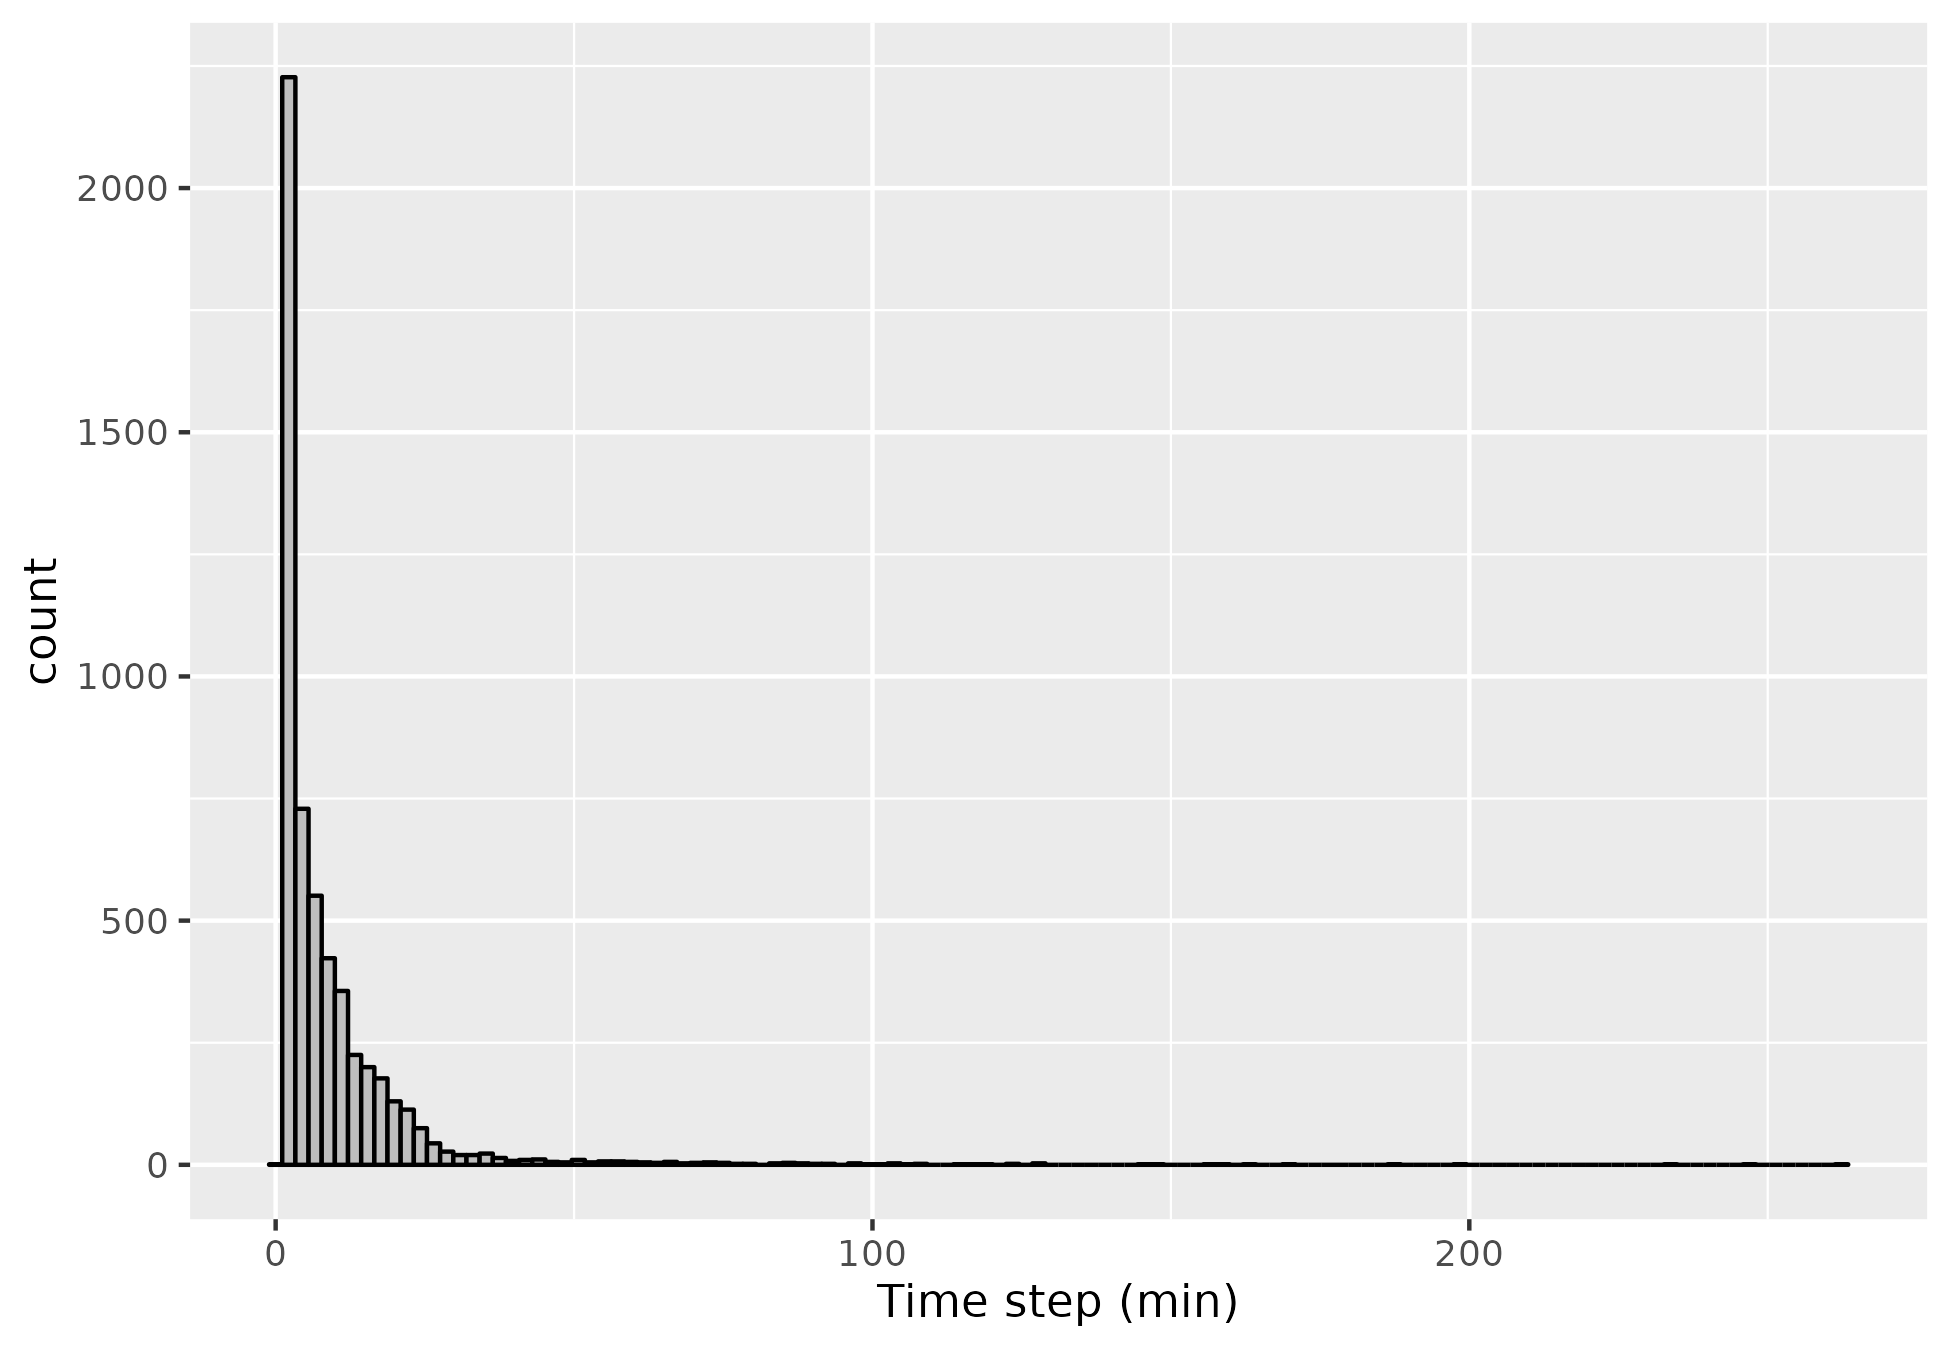
\includegraphics[scale=0.4]{images/data_exploration/all_time_steps_histo}
	\caption{Histogram of time steps}
	\label{fig:alltimestepshisto}
\end{figure}



The observations are divided into unexposed periods, for which the narwhals are not in line of sight with the ship; trial periods, when the narwhals are exposed to the ship and airguns are shot; and intertrial periods, when the narwhals are exposed to the ship but airguns are not shot. These periods are indicated by a categorical variable $T_{ship}$ in the dataset. Figure~\ref{fig: trials and intertrials distributions} shows how the exposure periods are distributed among the $6$ narwhals that were tracked. Our analysis in section 6 does not distinguish between intertrial and trial periods. They are both treated as exposure periods, though the nature and intensity of the behavioral response might differ for the two periods. We adopted this approach due to the lack of intertrial data as well as a potential persistence in time of the behavior shift due to airgun exposure during trial periods.

\begin{figure}[ht!]
	\centering
	\centering
	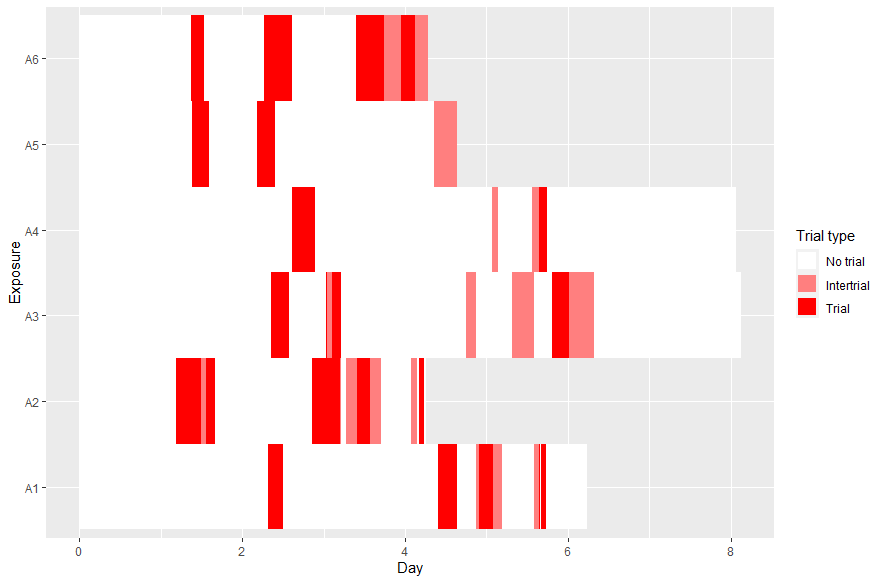
\includegraphics[scale=0.5]{images/data_exploration/trials.png}
	\caption{Trial and Intertrial periods for each narwhal}
	\label{fig: trials and intertrials distributions}
	
\end{figure}

Table~\ref{table: data distribution}  shows how the data is distributed among the different narwhals.
\begin{table}[ht!]
	\centering
	\begin{tabular}{|c|c|c|}
		\hline
		Narwhal ID & Number of measurement before exposure & Number of measurements during exposure \\
		\hline
		A1 & 354 & 576\\
		\hline
		A2  & 151 & 515 \\
		\hline
		A3 & 397 & 680 \\
		\hline
		A4 & 127 & 642  \\
		\hline
		A5 & 207 & 419\\
		\hline
		A6 & 322 & 425 \\
		\hline
		\textbf{Total} & \textbf{1558} & \textbf{3257} \\
		\hline
	\end{tabular}
	\caption{Distribution of the data among the 6 individuals}
	\label{table: data distribution}
\end{table}


The relevant covariates   used for the analysis of narwhals movement are summarized in Table \ref{tab: summary covariates}.



\begin{table}[ht!]
	\centering
	\begin{tabular}{|c|c|p{8cm}|c|}
		\hline
		Covariate & Unit & Description & Domain \\
		\hline
		$D^{ship}(t)$ & km & distance in kilometers between the narwhal and the ship at time $t$ & $\R^+$ \\
		\hline
		$E^{ship}(t)=\frac{1}{D^{ship}(t)}$ & $km^{-1}$ & global exposure level of the narwhal to the ship disturbance at time $t$ & $\R^+$ \\
		\hline
		$D^{shore}(t)$ & km & distance between the narwhal and the nearest point on the shore at time $t$ & $\R^+$ \\
		\hline
		$\Theta(t)$ & rad & angle between the vector that goes from the nearest shore point to the narwhal's position and the empirical velocity vector at time $t$  & $[-\pi,\pi]$ \\
		\hline 
	\end{tabular}
	\caption{Summary of the covariates}
	\label{tab: summary covariates}
\end{table}


\section{Proof of Proposition 3.1}
\label{section: transition density proof}

Here, we prove Proposition 3.1 The proof is inspired by the results in \citep{gurarie_correlated_2017,johnson_continuous_2008} and the proof of the transition density of the velocity process in \citep{albertsen_generalizing_2018}.
\begin{proof}
	The velocity process is an Ornstein-Uhlenbeck process. For $t \geq 0$ and $\Delta >0$,
	\begin{equation}
		V(t+\Delta)=\exp(-A\Delta) V(t)+ (I_2-\exp(-A\Delta))\mu +\frac{2\nu}{\sqrt{\pi \tau}}\int_{t}^{t+\Delta} \exp(A(s-(t+\Delta))) dW(s)
		\label{eq: RACVM solution}
	\end{equation}
	
	It has Gaussian transition density with mean 
	\begin{equation}
		\E(V(t+\Delta \vert V(t)))=\exp(-A\Delta) V(t)+ (I_2-\exp(-A\Delta))\mu 
	\end{equation}
	and covariance matrix 
	\begin{align*}Var(V(t+\Delta) \vert V(t))&=\frac{4\nu^2}{\pi \tau} \int_{t}^{t+\Delta} \exp(A(s-(t+\Delta))) \exp(A(s-(t+\Delta)))^{\top} ds\\
		&=\frac{4\nu^2}{\pi \tau} \int_{0}^{\Delta} \exp(-Au) \exp(-Au)^{\top} du 
	\end{align*}
	An integration by part gives 
	\[\int_{0}^{\Delta} \exp(-Au) \exp(-Au)^{\top} du =A^{-1}(I_2-\exp(-A\Delta))(I_2-\exp(-A\Delta))^\top A^{-\top}\]. In the sequel, we denote $S(\Delta)=A^{-1}(I_2-\exp(-A\Delta))$.
	Since $\exp(-Au)=\exp(-\frac{u}{\tau}) R_{-\omega u}$ where $R_{-\omega u}$ is the rotation matrix with angle $-\omega u$, we can deduce that the two components of the velocity are independent and have the same variance, denoted  $q_2(\Delta)$. This variance is 
	\begin{equation}
		q_2(\Delta)=\frac{2\nu^2}{\pi}\left(1-\exp\left(-\frac{2\Delta}{\tau}\right)\right).
	\end{equation}
	These results are found in \cite{gurarie_correlated_2017}.
	In the sequel, we  use the notation 
	\[\zeta(t,s) =\frac{2\nu}{\sqrt{\pi \tau}}\int_{t}^{s} \exp(A(u-s)) dW(u).\] 
	Using that $V(s)=\mu+\exp(-A(s-t))(V(t)-\mu)+\zeta(t,s)$, we have
\begin{align*}
    X(t+\Delta) &= X(t) + \int_t^{t+\Delta} V(s) \, ds \\
    &= X(t) + \mu \Delta + \int_t^{t+\Delta} \exp(-A(s-t))(V(t) - \mu) \, ds \\
    &\quad + \int_t^{t+\Delta} \zeta(t,s) \, ds \\
    % &= X(t) + \mu \Delta + \int_0^{\Delta} \exp(-As)(X(t) - \mu) \, ds + \int_t^{t+\Delta} \zeta(t,s) \, ds \\
    &= X(t) + \mu \Delta + \left(A^{-1}(V(t) - \mu) - A^{-1}\exp(-A\Delta)(X(t) - \mu)\right) \\
    &\quad + \int_t^{t+\Delta} \zeta(t,s) \, ds
\end{align*}
	Thus, 
	\begin{equation}
		X(t+\Delta)=X(t)+\mu \Delta+A^{-1} \left( I_2-\exp(-A\Delta)\right)(V(t)-\mu)+\xi(t,t+\Delta) 
	\end{equation}
	where $ \xi(t,t+\Delta)=\int_t^{t+\Delta} \zeta(t,s)ds$.
	The location process is also Gaussian with mean 
	\begin{equation}
		\E(X(t+\Delta) \vert V(t),X(t)) =X(t)+\mu \Delta+A^{-1} \left( I_2-\exp(-A\Delta)\right)(V(t)-\mu).
	\end{equation}
	To get an expression of the covariance matrix, first rewrite
	\begin{align*}
		\xi(t,t+\Delta)&=\int_t^{t+\Delta} \frac{2 \nu}{\sqrt{\pi \tau}} \left( \int_t^s \exp(-A((u-s))dW(u) \right) ds \\
		%&=\frac{2\nu}{\sqrt{\pi\tau}} \int_t^{t+\Delta} \left( \int_u^{t+\Delta} \exp(A(u-s)) ds \right) dW(u)  \\
		&= \frac{2\nu}{\sqrt{\pi \tau}} \int_t^{t+\Delta} (A^{-1}-A^{-1}\exp(A(u-t-\Delta))) dW(u) \\
		&= \frac{2\nu}{\sqrt{\pi \tau}} \int_t^{t+\Delta} A^{-1}(I_2-\exp(A(u-t-\Delta))) dW(u)
	\end{align*}
	Then use Ito's isometry
 \begin{align*}
    \mbox{Var}(X(t+\Delta)\vert X(t),V(t))&=\frac{4 \nu^2}{\pi \tau} 
    \int_{t}^{t+\Delta} A^{-1} (I_2-\exp(A(u-t-\Delta)))\\
    &\quad \times (I_2-\exp(A(u-t-\Delta)))^\top A^{-\top} \, du \\
    &=\frac{4 \nu^2}{\pi \tau} \int_{0}^{\Delta} A^{-1} (I_2-\exp(-Ar))\\
    &\quad \times (I_2-\exp(-Ar))^\top A^{-\top} \, dr.
\end{align*}
This integral can be computed explicitly since 
\[A^{-1} (I_2-\exp(-Ar))(I_2-\exp(-Ar))^\top A^{-\top}=\frac{1}{C} f(r) I_2 \]
where $f(r)=1-2\exp\left( -\frac{r}{\tau}\right)\cos(\omega r)+\exp\left(\frac{-2r}{\tau}\right)$ and $C=\frac{1}{\tau^2}+\omega^2$.
We obtain that $X_1(t+\Delta)$ and $X_2(t+\Delta)$ are independent and have the same variance, denoted $q_1(\Delta)$.
Writing $\sigma=\frac{2\nu}{\sqrt{\pi \tau}}$, the variance is
\begin{align*}
    q_1(\Delta) &= \frac{\sigma^2}{C} \left( \Delta 
    - 2 \frac{\omega \sin(\omega \Delta) - \frac{1}{\tau} \cos(\omega \Delta)}{\frac{1}{\tau^2} + \omega^2 } 
    \exp\left( -\frac{\Delta}{\tau} \right) \right. \\
    &\quad \left. + \frac{\tau}{2} \left( \frac{\omega^2 - \frac{3}{\tau^2}}{\frac{1}{\tau^2} + \omega^2} 
    - \exp\left( -\frac{2\Delta}{\tau}\right) \right) 
    \right)
\end{align*}
	
Now we compute the covariance between   $X$ and $V$ to get the full covariance matrix of $U$:
\begin{align*}
    \Gamma(\Delta) &= \frac{4\nu^2}{\pi \tau} \E\left(\left( \int_t^{t+\Delta} A^{-1}(I_2-\exp(A(u-t-\Delta))) \, dW(u)\right) \right. \\
    &\quad \left. \times \left(\int_{t}^{t+\Delta} \exp(A(s-(t+\Delta))) \, dW(s)\right)^\top\right) \\
    &= \int_t^{t+\Delta} A^{-1}(I_2-\exp(A(u-(t+\Delta)))) \exp(A(u-(t+\Delta)))^\top \, du \\
    &= \frac{4\nu^2}{\pi \tau} \int_0^{\Delta} A^{-1}(I_2-\exp(-Ar)) \exp(-Ar)^\top \, dr.
\end{align*}
	Then, 
	\[A^{-1}(I_2-\exp(-Ar)) \exp(-Ar)^\top=\frac{1}{C}\exp\left(-\frac{r}{\tau} \right) \begin{pmatrix} g(r) & h(r) \\ -h(r) & g(r) \end{pmatrix}\]
	where 
\begin{align*}
    g(r) &= \frac{1}{\tau} \left(\cos(\omega r) - \exp\left( -\frac{r}{\tau} \right)\right) 
    + \omega \sin(\omega r), \\
    h(r) &= -\frac{1}{\tau} \sin(\omega r) 
    + \omega \left(\cos(\omega r) - \exp\left( -\frac{r}{\tau}\right)\right).
\end{align*}
	Finally we get
	\[
	\gamma_1(\Delta)=\frac{\sigma^2}{2C}\left( 1+\exp\left( -\frac{2\Delta}{\tau}\right)-2\exp\left( -\frac{\Delta}{\tau}\right) \cos(\omega \Delta)\right),
	\]
	\[\gamma_2(\Delta)=\frac{\sigma^2}{C}\left( \exp\left( -\frac{\Delta}{\tau}\right) \sin(\omega \Delta)-\frac{\omega \tau}{2} \left(1-\exp\left( -2 \frac{\Delta}{\tau}\right) \right)\right).\]
	
	In the specific case $\omega=0$, we obtain $C=\frac{1}{\tau^2}$ and the variance of  $X$ becomes 
	\[q_1(\Delta)=\sigma^2 \tau^2\left( \Delta +2\tau\exp\left( -\frac{\Delta}{\tau}\right)+\frac{\tau}{2}\left( -3 -\exp\left( -\frac{2\Delta}{\tau}\right) \right)\right).
	\]
	Writing $\beta=\frac{1}{\tau}$ and reorganizing the terms, we obtain
	\begin{equation}q_1(\Delta)=\frac{\sigma^2}{\beta^2}\left(\Delta -2 \frac{1-\exp(-\beta \Delta)}{\beta}+\frac{1-\exp(-2\beta \Delta)}{2\beta}\right).
	\end{equation}
	This result match equation $(6)$ in \citep{johnson_continuous_2008}. Similarly, in the case $\omega=0$, we get $\gamma_2=0$ and the expression for $\gamma_1$ match equation $(7)$ in \citep{johnson_continuous_2008}.
	
\end{proof}

\section{Approximate transition density}

We now suppose that the angular velocity $\omega$ varies with time. Denote $\mathcal{A}(0,t)=\int_0^t A(s) ds$ the time integral of the drift matrix.
A similar calculation as before gives
\[V(t+\Delta)=\exp(-\mathcal{A}(t,t+\Delta)) V(t)+\sigma \int_t^{t+\Delta} \exp(-\mathcal{A}(s,t+\Delta)) dW(s)\]


Therefore, $V(t+\Delta) \vert V(t)$ is normally distributed with mean
\[\E(V(t+\Delta) \vert V(t))=\exp(-\mathcal{A}(t,t+\Delta)) V(t)\]
and covariance matrix 
\[\mbox{Var}(V(t+\Delta) \vert V(t))=\sigma^2\int_t^{t+\Delta} \exp(-\mathcal{A}(s,t+\Delta)) \exp(-\mathcal{A}(s,t+\Delta))^\top ds\]


The exact formula for the process $X$ is 
\[X(t+\Delta)=X(t)+\int_t^{t+\Delta} \exp(-\mathcal{A}(t,s)) V(t) ds +\sigma \int_t^{t+\Delta} \int_t^s \exp(-\mathcal{A}(u,s)) dW(u) ds \]
Consequently, the process is gaussian with mean given by
\[\E(X(t+\Delta) \vert X(t))=X(t)+\int_t^{t+\Delta} \exp(-\mathcal{A}(t,s)) V(t) ds\]
and covariance matrix 
\[\mbox{Var}(X(t+\Delta) \vert X(t))=\sigma^2 \int_t^{t+\Delta} \lbrace \int_u^{t+\Delta} \exp(-\mathcal{A}(u,s))ds \rbrace \lbrace \int_u^{t+\Delta} \exp(-\mathcal{A}(u,s)) ds \rbrace^\top du\]

Denote $U(t)=(X(t), V(t))$. It is a Markov process with transition density
\[U(t+\Delta) \vert U(t)=u \sim \mathcal{N}(T(\Delta) u, Q(\Delta))\]
where 
\begin{equation}
	T(\Delta) = \begin{pmatrix}
		I_2 & \int_t^{t+\Delta} \exp(-\mathcal{A}(t,s)) ds \\
		0_2 & \exp(-\mathcal{A}(t,t+\Delta))
	\end{pmatrix}
\end{equation}

\begin{equation}
	Q(\Delta) = \begin{pmatrix}
		
		Q_{11}(\Delta) & Q_{12}(\Delta)  \\
		Q_{21}(\Delta) &  Q_{22}(\Delta)
	\end{pmatrix}
\end{equation}
where 
\[Q_{11}(\Delta)=\sigma^2 \int_{t}^{t+\Delta} \left( \int_{u}^{t+\Delta} \exp(-\mathcal{A}(u,s)) ds \right) \left( \int_{u}^{t+\Delta} \exp(-\mathcal{A}(u,s)) ds \right)^\top du \]
\[Q_12(\Delta)=\sigma^2 \int_{t}^{t+\Delta} \left( \int_{u}^{t+\Delta} \exp(-\mathcal{A}(u,s)) ds \right) \exp(-\mathcal{A}(u,t+\Delta))^\top du\]
\[Q_{21}(\Delta)=Q_{12}(\Delta)^\top\]
\[Q_{22}(\Delta)=\sigma^2 \int_t^{t+\Delta} \exp(-\mathcal{A}(s,t+\Delta)) \exp(-\mathcal{A}(s,t+\Delta))^\top ds\]

Suppose we have approximations of the time varying matrix $A$ at times $t_0=t < t_1 < \cdots < t_n=t+\Delta$ and denote $\Delta_i=t_{i+1}-t_i$ for $i \in \{0,\cdots,n-1\}$.
Then we can approximate
\[\exp(-\mathcal{A}(t,t+\Delta))=\prod_{i=0}^{n-1} \exp(-A_i\Delta_i)\]
where $A_i=A(t_i)$. Each matrix $\exp(-A_i\Delta_i)$ is a weighted rotation matrix with angle $-\omega_i\Delta_i$.
For conciseness, in the sequel we denote $E_i=\exp(-A_i\Delta_i)$, $P_{jk}= \prod_{i=j}^{k-1} E_i$ and $S_j=S(\Delta_j)$.

The covariance matrix of $V$ is approximated by 
\[Q_{22}(\Delta)\simeq\sum_{j=0}^{n-1} \sigma^2 P_{j+1,n} P_{j+1,n}^\top S_j S_j^\top\]
The mean for the process $X$ can be estimated with the following formula
\[\E(X(t+\Delta) \vert X(t)) \simeq X(t)+\sum_{k=0}^{n-1} P_{0,k} S_k  V(t) \]
The covariance can also be approximated. The first step is to approximate $\mathcal{A}(u,s)$ for $u \in [t,t+\Delta]$ and $s \in [u,t+\Delta]$. For a fixed $u \in [t_{j-1},t_j]$, 

\begin{align*}
	& \exp(-\mathcal{A}(u,s)) \simeq 
	\exp(-A_{j-1}(t_j-u)) \1_{[u,t_j]}(s) +\\
	& \sum_{k=j}^{n-1} \exp(-A_{j-1}(t_j-u)) \times \prod_{i=j}^{k-1} \exp(-A_i \Delta_i) \times \exp(-A_k (s-t_k)) \1_{[t_k,t_{k+1}]}(s)
\end{align*}

This gives the following approximation for any $u \in [t_{j-1},t_j]$
\begin{align*}
	&\int_u ^{t+\Delta} \exp(-\mathcal{A}(u,s)) ds \simeq A_{j-1}^{-1} (I_2-\exp(-A_{j-1} (t_j-u)))+ \\
	&\sum_{k=j}^{n-1} \exp(-A_{j-1} (t_j-u)) \prod_{i=j}^{k-1} \exp(-A_i \Delta_i) A_k^{-1} (I_2- \exp(A_k \Delta_k)) 
\end{align*}
We then deduce an approximation of the covariance matrix.

\begin{align*}
	\mbox{Var}(X(t+\Delta) \vert X(t)) \simeq &\sum_{j=1}^n \sigma^2 A_{j-1}^{-1} A_{j-1}^{-\top}(\Delta_{j-1} I_2-S_{j-1}-S_{j-1}^\top + S_{j-1}S_{j-1}^\top) \\
	&+ \sigma^2  M_{jn}^\top A_{j-1}^{-1} (S_{j-1}^\top -S_{j-1} S_{j-1}^\top)M_j M_j^\top + \sigma^2  M_{jn} A_{j-1}^{-\top} (S_{j-1} -S_{j-1} S_{j-1}^\top) \\
	&+M_{jn} M_{jn}^\top S_{j-1} S_{j-1}^\top 
\end{align*}

where $M_{jn} = \sum_{k=j}^{n-1} P_{jk} S_k $.


Finally, we have the following formula to approximate the covariance matrix between $X$ and $V$.

\begin{align*}
	\mbox{Var}(X(t+\Delta),V(t+\Delta) \vert X(t),V(t))=& \sum_{j=1}^n \sigma^2 P_{j,n}^\top A_{j-1}^{-1}(S_{j-1}^\top-S_{j-1} S_{j-1}^\top)  
	+\sigma^2 M_{jn} P_{j,n}^\top S_{j-1} S_{j-1}^\top 
\end{align*}

We denote
\[\tilde{T}_n=\begin{pmatrix} I_2 & \sum_{k=0}^{n-1} P_{0,k} S_k \\
	0_2  &  \prod_{i=0}^{n-1}  E_i \end{pmatrix}
\]
and \[\tilde{Q}_n = \begin{pmatrix}  \tilde{Q}_n^{11}& \tilde{Q}_n^{12} \\
	\tilde{Q}_n^{21}& \tilde{Q}_n^{22} \end{pmatrix}\]
where 
\begin{align*}
	\tilde{Q}_n ^{11}=&\sum_{j=1}^n \sigma^2 A_{j-1}^{-1} A_{j-1}^{-\top}(\Delta_{j-1} I_2-S_{j-1}-S_{j-1}^\top + S_{j-1}S_{j-1}^\top) \\
	&+ \sigma^2  M_{jn}^\top A_{j-1}^{-1} (S_{j-1}^\top -S_{j-1} S_{j-1}^\top) + \sigma^2  M_{jn} A_{j-1}^{-\top} (S_{j-1} -S_{j-1} S_{j-1}^\top) \\
	&+\sigma^2M_{jn} M_{jn}^\top S_{j-1} S_{j-1}^\top \\
	\tilde{Q}_n ^{12}=&\sum_{j=1}^n \sigma^2 P_{j,n}^\top A_{j-1}^{-1}(S_{j-1}^\top-S_{j-1} S_{j-1}^\top)  
	+\sigma^2 M_{jn} P_{j,n}^\top S_{j-1} S_{j-1}^\top \\
	\tilde{Q}_n ^{21}=&(\tilde{Q}_n ^{12})^\top \\
	\tilde{Q}_n^{22} = & \sum_{j=0}^{n-1} \sigma^2 P_{j+1,n} P_{j+1,n}^\top S_j S_j^\top
\end{align*}
We can express $\tilde{T}_n$ and $\tilde{Q}_n$ in terms of the elementary matrices 
\[T_i=\begin{pmatrix} I_2 & S_i \\ 0_2 & E_i \end{pmatrix}  \mbox {and } 
Q_i=\begin{pmatrix} \sigma^2 A_i^{-1}A_i^{-\top} ( \Delta_iI_2-S_i-S_i^\top+S_iS_i^\top) & \sigma^2 A_i^{-1} (S_i^\top-S_iS_i^\top) \\
	\sigma^2 A_i^{-\top} (S_i-S_iS_i^\top) & \sigma^2 S_i S_i^\top
\end{pmatrix}
\]

\begin{equation}
	\tilde{T}_n = T_{n-1} \times \cdots \times T_1 \times T_0
	\label{eq: approximate link matrix}
\end{equation}
\begin{equation}
	\tilde{Q}_n= \sum_{k=1}^{n-1} T_{n-1}^\top \cdots T_{k+1}^\top Q_k T_{k+1} \cdots T_{n-1}
\end{equation}

\begin{proof}
	$\tilde{T}_n=T_0$ and $\tilde{Q}_1=Q_0$. Then, for $n \geq 2$, 
	\begin{align*}
		\tilde{T}_{n}=&\begin{pmatrix} 
			I_2 & P_{0,n-1}S_{n-1}+\sum_{j=0}^{n-2} P_{0,j} S_j \\
			0_2 & P_{0,n} E_{n-1}
		\end{pmatrix}
	=\begin{pmatrix}
		I_2 & S_{n-1} \\
		0_2 & E_{n-1}
	\end{pmatrix}
	\begin{pmatrix} 
	I_2 & \sum_{j=0}^{n-2} P_{0,j} S_j \\
	0_2 & P_{0,n-1}
	\end{pmatrix}\\
	&= T_{n-1} \tilde{T}_{n-1}
	\end{align*}
Then, using that $M_{n,n}= 0_2 $ and $P_{n,n}=I_2$ we get
\[ \tilde{Q}_n=Z_{n-1}+Q_{n-1} \]
where 
\[Z_{n-1}=\begin{pmatrix} \sum_{j=1}^{n-1} Q_{j-1}^{11} +M_{jn}^\top Q_{j-1}^{12}+M_{jn} Q_{j-1}^{21}+M_{j,n}M_{j,n}^\top Q_{j-1}^{22} & \sum_{j=1}^{n-1}  P_{j,n}^\top Q_{j-1}^{12} +M_{j,n} P_{j,n}^\top Q_{j-1}^{22} \\
	\sum_{j=1}^{n-1} P_{j,n} Q_{j-1} ^{21} + M_{jn}^\top P_{jn} Q_{j-1}^{22} & \sum_{j=1}^{n-1} P_{jn}^\top P_{jn} Q_{j-1}^{22}
	\end{pmatrix}
\]
Then, since $M_{j,n}=M_{j,n-1}+P_{j,n-1} S_{n-1}$ we get
\begin{align*} Z_{n-1}=\begin{pmatrix} \tilde{Q}_{n-1}^{11}+S_{n-1}^\top Q_{n-1}^{12}+S_{n-1} \tilde{Q}_{n-1}^{21}+S_{n-1}S_{n-1}^\top \tilde{Q}_{n-1}^{22} &  E_{n-1}^\top \tilde{Q}_{n-1}^{12}+E_{n-1}^\top S_{n-1} \tilde{Q}_{n-1}^{12}\\
		E_{n-1} \tilde{Q}_{n-1}^{21}+E_{n-1} S_{n-1}^\top \tilde{Q}_{n-1}^{22} & E_{n-1}E_{n-1}^\top
	\end{pmatrix}
\end{align*}
And this is equal to $T_{n-1}^\top \tilde{Q}_{n-1} T_{n-1}$.
	
\end{proof}

\section{Measurement error}

In the application in Section 6, different values of the measurement error were estimated for the data before and after exposure: $35$ m before and $48$ m after. Both these values are consistent with the results in \citep{wensveen_path_2015}. However, the post exposure estimation gave non-positive definite Hessian matrix for the negative log-likelihood, which prevents from using the information matrix equality to get confidence intervals of the estimates. Fixing a $35$ m measurement error value when fitting the response model led to the same issue. We therefore tried different values of the measurement error, and kept the one that gave a positive definite hessian matrix and had the highest log-likelihood value. It turned out to be $50$ m, very close to the initially estimated $48$ m. Table~\ref{tab: estimates for fixed measurement errors} shows these results. In comparison, the final values of the log-likelihood when $\sigma_{obs}$ is estimated from the data are respectively $4273$ and $8043$ before and after exposure, while the estimate of $\tau_0$ is $1.10$, and the estimates of $\alpha_\tau$ and $\alpha_\nu$ are respectively $-4.19$ and $0.66$, which is in the confidence interval of the final estimations we kept (those obtained for $\sigma_{obs}=50$ m).
\begin{table}[ht!]
	\centering
	\begin{tabular}{|c|c|c|c|c|c|c|}
		\hline
		$\sigma_{obs}$ (m) & $\hat{\tau_0}$ & Baseline llk & Response llk & P.d hessian & $\alpha_{\tau}$ & $\alpha_\nu$ \\
		\hline
		$30$  & $0.96 \pm 0.15$ & $4261$  & 8038 & No & $0.29$ & $2.17$ \\
		\hline
		$40$  & $1.18 \pm 0.16$   & $4266$ & 8014  & No  & $-2.06$ & $0.60$\\
		\hline
		$45$  & $1.29 \pm 0.17$   & $4243$ & 7965  & No & $-3.64$ & $0.49$\\
		\hline
		$\mathbf{50}$  & $\mathbf{1.35 \pm 0.16}$ & $\mathbf{4208}$ & $\mathbf{7861}$ & \textbf{Yes} & $\mathbf{-3.43 \pm 0.70}$ & $\mathbf{0.74 \pm 0.27}$\\
		\hline
		$75$ &  $1.63 \pm 0.19$ & $3944$ & $7225$ & Yes & $-3.88 \pm 0.73$ & $0.76 \pm 0.30$\\
		\hline 
		$100$ & $1.85 \pm 0.22$ & $3640$ & $6590$ & Yes & $-4.27 \pm 0.74$ & $0.63 \pm 0.29$ \\
		\hline 
	\end{tabular}
	\caption{Estimate for the baseline and response models for several fixed measurement errors.}
	\label{tab: estimates for fixed measurement errors}
\end{table}

\section{Code example}

We illustrate briefly how to fit our baseline SDE model and obtain the results with \texttt{smoothSDE} R package \cite{michelot_varying-coefficient_2021}. The version of the package including our new model is available \href{https://github.com/alexandre-delporte/smoothSDE}{here} . We suppose the package has been loaded. We consider a dataframe \texttt{dataBE} containing the preprocessed observations before exposure to the ship in the columns \texttt{x} and \texttt{y}, an animal identifier in a column \texttt{ID} and columns \texttt{Ishore} and \texttt{AngleNormal} for the covariates $I^{shore}$ and $\Theta$. The first step consists in choosing initial SDE parameters and model formulas. For the model we consider, there are five parameters $\mu_1$, $\mu_2$, $\tau$, $\nu$, and $\omega$, and each of them needs a formula. Specification of the formulas is identical to the \texttt{R} package \texttt{mgcv}. Among the parameters, $\mu_1$, $\mu_2$ will be set to 0, while $\tau$, $\nu$ and $\omega$ are expressed as in section 4.1.



\begin{lstlisting}[language=R]
#number of observation
n_pre<-nrow(dataBE)

#initial parameters
par0 <- c(0,0,1,4,0)

#model formulas
formulas <- list(mu1 = ~1 ,mu2 =~1,tau =~s(ID,bs="re"),nu=~s(ID,bs="re"),
omega=~ti(AngleNormal,k=5,bs="cs")+ti(Ishore,k=5,bs="cs")+
ti(AngleNormal,Ishore,k=c(5,5),bs="cs"))
\end{lstlisting}

We then specify the measurement error for each observation in an array of covariance matrices. We suppose they are all diagonal with the same standard deviation \texttt{sigma\_obs}. We will fix this measurement error. \\

\begin{lstlisting}[language=R]
# 50m measurement error
sigma_obs=0.05
H=array(rep(sigma_obs^2*diag(2),n_pre),dim=c(2,2,n_pre))
\end{lstlisting}

We can then create the SDE object as in \cite{michelot_varying-coefficient_2021}. We choose the type of SDE in the argument \texttt{type}. Here, it is \texttt{RACVM} (see Section 3.1) since we want to include a non zero rotation parameter $\omega$. The name of the columns where the observations are found is specified in the \texttt{response} argument.
We specify the measurement error matrix \texttt{H} in the argument \texttt{other\_data}. Fixed parameters are indicated in the argument \texttt{fixpar}.

\begin{lstlisting}[language=R]
#create SDE object
baseline_50m<- SDE$new(formulas = formulas,data = dataBE,type = "RACVM",
response = c("x","y"),par0 = par0,other_data=list("H"=H),
fixpar=c("mu1","mu2"))
\end{lstlisting}

To fix specific parameters in the statistical model, we need to use the \texttt{map} attribute. Here we use it to specify that the smoothing parameters should be fixed. Then we update the smoothing parameters to $1$, and fit the SDE model.

\begin{lstlisting}[language=R]
#update map to fix smoothig parameters
baseline_50m$update_map(list("log_lambda"=factor(c(1,2,rep(NA,4))))

#update smoothing parameters values
init_lambda=rep(1,6)
baseline_50m$update_lambda(init_lambda)

#fit the model
baseline_50m$fit()
\end{lstlisting}

The results of the optimization are stored in the attribute \texttt{tmb\_rep}.
We can extract the estimated parameters along with the standard errors.

\begin{lstlisting}[language=R]
#estimates
estimates_bas_50m=as.list(baseline_50m$tmb_rep(),what="Est")
#standard error
std_bas_50m=as.list(baseline_50m$tmb_rep(),what="Std")
\end{lstlisting}

Finally, we would like to plot all the smooth parameters as a function of the covariates. 
We can do it with the \texttt{get\_all\_plots} method.
We only need to specify the range of each covariate value we want to plot, a link function if we don't want to have directly the covariate on the x-axis but rather a function of the covariate, and the x-axis label of the plots. We put the option \texttt{show\_CI="pointwise"} to show the pointwise confidence intervals on the plots.

\begin{lstlisting}[language=R]
#range of the covariates
D_low=0.073
D_up=3
xmin=list("Ishore"=1/D_up)
xmax=list("Ishore"=1/D_low)
#link function
link=list("Ishore"=(\(x) 1/x))
#label
xlabel=list("Ishore"="Distance to shore")

#draw plots
plots_bas_50m=baseline_50m$get_all_plots(model_name="baseline_50m",
xmin=xmin,xmax=xmax,link=link,xlabel=xlabel,show_CI="pointwise",save=TRUE)
\end{lstlisting}


%%%%%%%%%%%%%%%%%%%%%%%%%%%%%%%%%%%%%%%%%%%%%%%%%%%%%%%%%%%%%
%%                  The Bibliography                       %%
%%                                                         %%
%%  imsart-nameyear.bst  will be used to                   %%
%%  create a .BBL file for submission.                     %%
%%                                                         %%
%%  Note that the displayed Bibliography will not          %%
%%  necessarily be rendered by Latex exactly as specified  %%
%%  in the online Instructions for Authors.                %%
%%                                                         %%
%%  MR numbers will be added by VTeX.                      %%
%%                                                         %%
%%  Use \citep{...} to cite references in text.             %%
%%                                                         %%
%%%%%%%%%%%%%%%%%%%%%%%%%%%%%%%%%%%%%%%%%%%%%%%%%%%%%%%%%%%%%

\bibliographystyle{imsart-nameyear} % Style BST file
\bibliography{biblio-supp}       % Bibliography file (usually '*.bib')
\end{document}
